\newpage

\section{General administration}
In this chapter, there is mostly reading. There are some questions that can be useful to answer. This chapter contains information about:
\begin{itemize}
    \item Adding a user.
    \item Adding a user to a group.
    \item Connecting using SSH without a password.
    \item How to reset your password.
    \item How to get a short description of what options does.
    \item How to update/upgrade your firewall.
    \item How to create a backup or restore a configuration.
    \item Enable/disable individual rules.
    \item Create an alias.
    \item Use the \cmd{PING} command from the firewall interface.
    \item Disable all packet filtering.
\end{itemize}

Use it as an encyclopedia if you get stuck on some of the topics in this chapter.

\subsection{User and Groups} \label{user_groups}
You can add users, and users can be added to a group. A normal security strategy is that a user only has access to their level of usage. Therefore you should not use a root account if you do not need to have root access to what you are doing. With that said, you will need a root account to perform the configurations that we are going to do in this tutorial.

If you need to create users, follow the configuration below:

\setupblock{\begin{enumerate}
    \item Go to \cmd{System -> Access -> Users}.
    \item Click \cmd{Add} to create a new user.
    \item Set \cmd{Username} and \cmd{Password} for the user.
    \item Set the \cmd{Full name} and \cmd{Email} for the user.
    \item Set the \cmd{Expiration date} for the user. If this field is \cmd{blank}, the user will never expire. This should be avoided. When date is set, it uses the format: \cmd{mm/dd/yyyy}.
    \item Configure \cmd{Group Memberships}. If groups do not exist, go to the next configuration below.
    \item Click the checkbox \cmd{Certification} if a user certificate should be created.
    \item If any authentication method other than username and a password is going to be used, insert the keys that should be used or create an internal certificate. (\cmd{OTP seed}, \cmd{Authorized keys} (section \ref{ssh_password}) or \cmd{IPsec Pre-Shared Key})
\end{enumerate}}

If you need to create groups, follow the configuration below:

\setupblock{\begin{enumerate}
    \item Go to \cmd{System -> Access -> Groups}.
    \item Click \cmd{Add} to create a new group.
    \item Give the new group a name and a description.
    \item Move user(s) to the group in the \cmd{Group memberships} part of the configuration.
\end{enumerate}}

\subsection{Login using SSH without password} \label{ssh_password}
% TODO something about what a private and public key are and what they are used to?
\opnsense\ comes with an OpenSSH server as default after you have set it up. The first step is to create a key pair for your client. When creating a key pair it is important to choose the correct key size. NIST (National Institute of Standards and Technology) is recommending at least 2048 bit as a minimum (\cite{Barker}). 

Follow the instructions below depending on what operating system you are using as your client:

\Linblock{\begin{enumerate}
    \item Check if the SSH client is installed using the command \cmd{ssh}. If it is successful, you will get a message with the different options you can use. If you do not have it installed, install it using the command \cmd{sudo apt install openssh-client}. 
    \item \cmd{ssh-keygen -t rsa -b 4096} to create the key-pair. When prompt, input your password and where you want to save it.
    \item Go to the common step below.
\end{enumerate}}
\vspace{-0.8cm}
\Winblock{\begin{enumerate}
    \item Check if you have the SSH client on your system using the command \cmd{ssh}. If it is successful you will get a message with the different options you can use. If you do not have it installed, install it via the add/remove windows functions or use the Windows Store.
    \item \cmd{ssh-keygen -b 4096} to create the key-pair. When prompt, input your password and where you want to save it.
    \item Go to the common step below the Linux step.
\end{enumerate}}

The next step is to get your public key to the \opnsense\ firewall.

\setupblock{Common step:
\begin{enumerate}
    \item Go to your \opnsense\ web GUI and \cmd{System -> Access -> Users}.
    \item Click on the edit button (a pencil on the right side of the user name) and add your public key in the \cmd{Authorized keys}. Make sure your public key is on one line.
    \item Test from your client if you can log in using passwordless SSH.
\end{enumerate}}

\warnblock{If you get problems adding the ssh key, make sure the key is on \Rtext{one line}.}

% TODO insert picture?

\quesblock{\begin{enumerate}
    \item[8.] What is key-size?
    \item[9.] What is the difference between a private key and a public key? 
\end{enumerate}}

\subsection{Password reset}
There are three different methods that can be used depending on if the \cmd{Password protect the console menu} is set in \cmd{System -> Settings -> Administration} in the web GUI (Graphical User Interface) (figure \ref{opensense:password_protect_CLI}) or if you have access to the web GUI at all.

\begin{itemize}
    \item Method one can be used when you have access to the web GUI.
    \item Method two is only going to work if the \cmd{Password protect the console menu} checkbox is not checked and you do not have access to the web GUI.
    \item Method three is only going to work if the \cmd{Password protect the console menu} checkbox is checked.
\end{itemize}

\begin{figure}[h!]
    \centering
    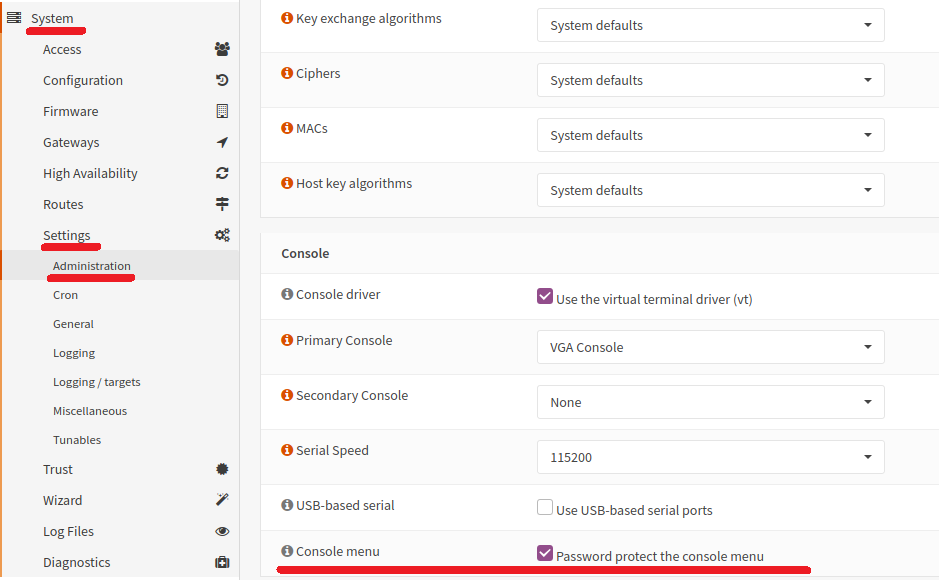
\includegraphics[width=0.5\textwidth]{Images/opensense_system_settings_administration_protect_cli.PNG}
    \caption{\opnsense\ Password protect the console menu checkbox}
    \label{opensense:password_protect_CLI}
\end{figure}

\subsubsection*{Method 1:}
Using the web GUI, go to \cmd{Lobby -> Password}, enter your new password, retype (confirm) it and click on \cmd{Save} to confirm, and set the new password.

\subsubsection*{Method 2:}

\begin{importantblock}
    Method two is only going to work if the checkbox \cmd{Password protect the console menu} is not checked and you do not have access to web GUI. If you do not know, if the \cmd{Password protect the console menu} is checked, go to method \ref{method3} instead.
\end{importantblock}

Start your \opnsense\ firewall and wait for it to start completely. Then login\footnote{root:opnsense (Username and password if you did not change it)} using the CLI. After you have logged in, you should see a screen similar to figure \ref{cli:login_root}. Choose option 3, and change your password.

\begin{figure}[h!]
    \centering
    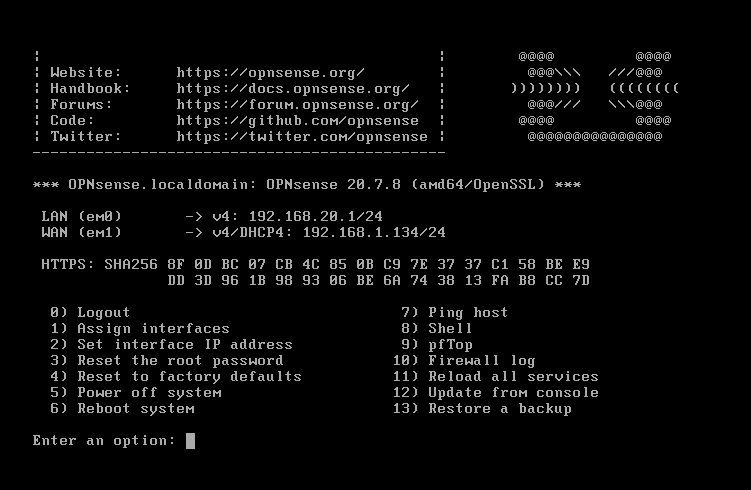
\includegraphics[width=0.5\textwidth]{Images/cli_login_root.PNG}
    \caption{\opnsense\ login screen CLI}
    \label{cli:login_root}
\end{figure}

\subsubsection*{Method 3:} \label{method3}

\setupblock{
\begin{enumerate}
    \item Reboot and when the boot menu is displayed after the reboot, choose the \cmd{Boot Single User} option.
    \item You are now presented with a CLI with the question: \cmd{Enter full pathname of shell or RETURN for /bin/sh}. Hit the \Rtext{ENTER}\ key to get the default shell.
    \item Mount the disk using the command \cmd{mount -o rw /}
    \item Write this file path in your shell: \cmd{/usr/local/opnsense/scripts/shell/password.php}. This will ask if you want to continue and answer with the command \cmd{y}.
    \item Type your new password twice when asked for it.
    \item Reboot
    \item Log in as normal using your new password. The new password will work in CLI, SSH and, via the web portal.
\end{enumerate}}

\quesblock{\begin{enumerate}
    \item[10.] What does the \cmd{Password protect the console menu} checkbox in \cmd{System -> Settings -> Administration} in the web GUI do?
\end{enumerate}}

\subsection{Get help} \label{get_help}
Many of the variables/options that can be set during your work with \opnsense\ have a short description that can help you to understand better what it does. If it exists, there will be an icon in the right top corner, below the search bar, that can be clicked. It is activated when it has a green colour. This can be seen in figure \ref{opensense:get_help}.

\begin{figure}[h!]
    \centering
    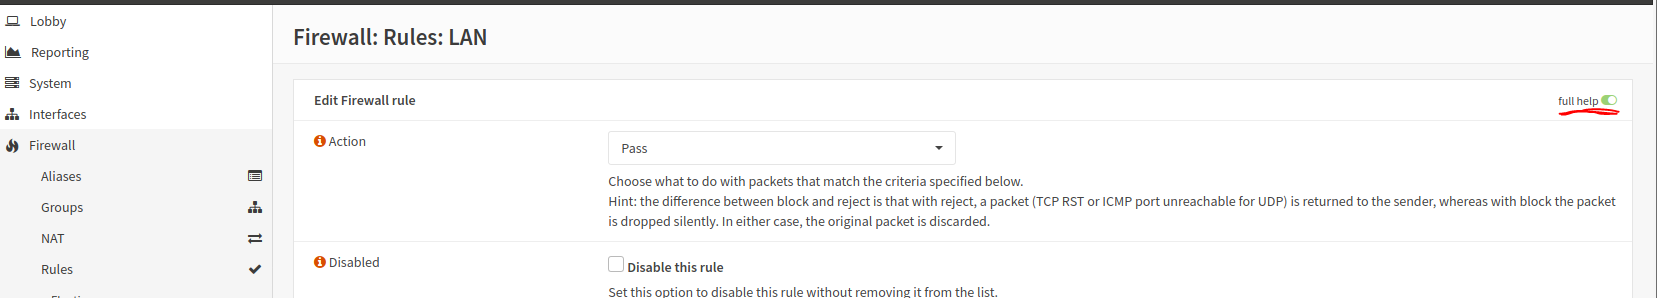
\includegraphics[width=0.9\textwidth]{Images/firewall/help.PNG}
    \caption{\opnsense\ Help}
    \label{opensense:get_help}
\end{figure}

\subsection{Update, upgrade, and plugins}
In \cmd{System --> Firmware} it is possible to update and upgrade the different packages, plugins, and the firmware itself. This is also the place where new plugins are installed from.

\subsection{Backup / restore of configuration}
Backup and restore is done in the menu: \cmd{System --> Configuration --> Backups}. To download the backup configuration file, click on the \cmd{Download configuration} button and save it to your disk. And when restoring the configuration, click on the \cmd{Restore configuration} button and choose the configuration file you want to use.

When downloading a configuration file, there is a checkbox option to protect it from unauthorized usage. And the same exist for restoring an encrypted configuration file.

\warnblock{Please, make backups of your configuration before you are starting with another topic in this tutorial. It will make it is easy to restore to an earlier point that you know is working.}

\subsection{Enable / disable individual rules}
Most rules have a checkbox that can be used to enable the rule (see figure \ref{opensense:admin_enable}). If it has a checkmark, it is enabled.

\begin{figure}[h!]
    \centering
    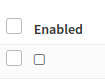
\includegraphics[width=0.15\textwidth]{Images/admin/enable.PNG}
    \caption{Enable / disable rules}
    \label{opensense:admin_enable}
\end{figure}

\subsection{Alias}
An alias is used for items that are bundled together using one name. An alias can, for example, contain off hosts, networks, or ports (for the full list, see table \ref{tab:alias_types}). The main reason for the usage of aliases is to make, for example, the list of firewall rules easier to read. If the aliases are used, one rule can be used for something that affects multiple hosts. To create an alias:

\setupblock{
    \begin{enumerate}
        \item Go to \cmd{Firewall --> Aliases}.
        \item Click the \cmd{+} button on the right side of the screen.
        \item Give the alias a name in the \cmd{Name} field.
        \item Chose the type you want to use.
        \item And the \cmd{Content} field is where you type in, for example, the IP, hostname, or port.
        \item Give the alias a description in the \cmd{Description} field.
    \end{enumerate}
}


\begin{table}[h!]
    \begin{center}
    \begin{tabular}{|l|l|}
    \hline
    \textbf{Type:} & \textbf{Description:} \\ \hline
    Hosts & IP or FQDN (Fully Qualified Domain Name). \\ \hline
    Networks & A network range with CIDR added at the end. \\ \hline
    Ports & Port number or port range (divided with a \cmd{:}). \\ \hline
    MAC addresses & Partial or full mac address. \\ \hline
    URL (IPs) & one or multiple IPs. \\ \hline
    URL Tables (IPs) & one or multiple IPs. \\ \hline
    GeoIP & Country or region. \\ \hline
    Network group & A combination of different types. \\ \hline
    External (advanced) & Alias that is managed externally. \\ \hline
    \end{tabular}
    \caption{Full list of what an alias can consist of}
    \label{tab:alias_types}
    \end{center}
\end{table}

\tipbox{The character \cmd{!} can be used to exclude items from an alias.}

\subsection{Troubleshooting}
In this section, there are some troubleshooting tips and tricks that you can use if you get problems. In the \cmd{Interfaces --> Diagnostics} menu, there are multiple tools that can be used to find an error during troubleshooting. In the following bullet point list, there is a short overview of the different tools and what they can be used for.

\begin{itemize}
    \item ARP table - The ARP table (Address Resolution Protocol) is a table over all known network IP's and MAC ( Media Access Control) addresses that are connected to the firewall.
    \item DNS lookup - Can resolve IPs or hostnames to a domain.
    \item NDP table - The NDP (Neighbor Discovery Protocol) table shows addresses that are learned for IPv6.
    \item Netstat - Shows status information about interfaces, protocol, sockets, netisr, memory, and bpf.
    \begin{itemize}
        \item Interfaces - Contains information about each interface. This could be both physical or virtual interfaces. Metrics shown is number of packets, bytes sent/recived.
        \item Protocol - Contains statistical information for multiple protocols. Examples of statistics it show is number of tcp listening connections, sent packets, duplicate packets, etc, etc.
        \item Sockets - Combines the \cmd{netstat}\footnote{\url{https://www.freebsd.org/cgi/man.cgi?query=netstat&sektion=1}} with \cmd{sockstat}\footnote{\url{https://www.freebsd.org/cgi/man.cgi?query=sockstat&sektion=1&format=html}} in FreeBSD and produce statistics about processes that are listening.
        \item Netisr - Show statistics from the kernel network dispatch service, known as \cmd{netisr(9)}\footnote{\url{https://www.freebsd.org/cgi/man.cgi?format=html&query=netisr(9)}}.
        \item Memory - Shows information from the memory management routines (\cmd{mbuf(9)}\footnote{\url{https://www.freebsd.org/cgi/man.cgi?query=mbuf&sektion=9&format=html}}).
        \item Bpf - Shows statistics from \cmd{bpf(4)}\footnote{\url{https://www.freebsd.org/cgi/man.cgi?bpf(4)}}.
    \end{itemize}
    \item Packet Capture - See section \ref{pk_capture}
    \item Ping - See section \ref{ping}
    \item Port Probe - Can be used to test if a port is open.
    \item Trace Route - Can be used to follow a route. Lists all the IPs in the route.
\end{itemize}

\subsubsection{Ping} \label{ping}
The \cmd{ping} command is very useful when you are trying to find errors in your network setup. To use the ping command, follow the instructions below:

\setupblock{
    \begin{enumerate}
        \item Go to \cmd{Interface --> Diagnostics --> Ping}.
        \item Set \cmd{Host} to the address (or IP) you want to ping.
        \item Set \cmd{Source Address} to the interface that should be used.
        \item Set \cmd{Count} to how many ping requests you want to send.
    \end{enumerate}
}

\quesblock{\begin{enumerate}
    \item[11.] Try to ping your client. Do you get something similar to figure \ref{opensense:admin_ping}?
\end{enumerate}}

\begin{figure}[h!]
    \centering
    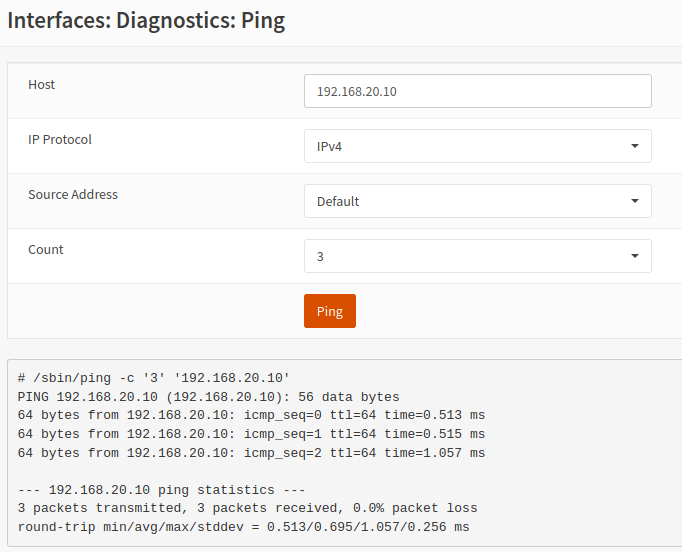
\includegraphics[width=0.55\textwidth]{Images/admin/ping.PNG}
    \caption{\cmd{ping} command}
    \label{opensense:admin_ping}
\end{figure}

\subsubsection{Disable all packet filtering} \label{pk_capture}
Another feature that could help you during troubleshooting is to disable packet filtering temporarily. 
\begin{importantblock}
    This will allow everything through your firewall. Be careful if you choose to do this in a production environment! Remember to \Rtext{enable} this feature when you are done with troubleshooting.
\end{importantblock}

\setupblock{
    \begin{enumerate}
        \item Go to \cmd{Firewall --> Settings --> Advanced}.
        \item Scroll down and find \cmd{Disable Firewall}, figure \ref{opensense:admin_disable_firewall}.
        \item Click the checkmark and the \cmd{Save} button at the bottom.
    \end{enumerate}
}

\begin{figure}[h!]
    \centering
    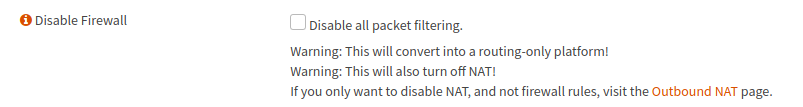
\includegraphics[width=0.8\textwidth]{Images/admin/firewall_disable_packet_filtering.PNG}
    \caption{Disable Firewall}
    \label{opensense:admin_disable_firewall}
\end{figure}
